\documentclass[oneside,english,titlepage]{scrbook}
\usepackage[T1]{fontenc}
\setcounter{secnumdepth}{3}
\setcounter{tocdepth}{3}
\usepackage{babel}
\usepackage{fancybox}
\usepackage{calc}
\usepackage{pifont} %For ding marks, http://willbenton.com/wb-images/pifont.pdf
\usepackage{textcomp}
\usepackage{xcolor}
\usepackage{enumitem}
\usepackage{graphicx}
\usepackage{booktabs}
\usepackage[unicode=true]
 {hyperref}

 %Own colors:
\definecolor{ownRed}{rgb}{0.858, 0.188, 0.478}
\definecolor{ownGreen}{rgb}{0.073, 0.532, 0.062}
\definecolor{ownOrange}{rgb}{0.6,0.6,0.0}

 %Own commands for own symbols:
\newcommand{\completeValue}{\textcolor{ownGreen}{\ding{51}}}
\newcommand{\noneValue}{\textcolor{ownRed}{\ding{55}}}
\newcommand{\partialValue}{\textcolor{ownOrange}{\ding{120}}}





\begin{document}

\title{Students Management System}
% The title of the memory can be different to the name of the
% application. For instance, SMS, a process accelerator for
% educational centers.

\subtitle{Proccess accelerator for educational centers}
% Check spelling. And then again, Check spelling - JJ

\subtitle{Juan Antonio Fern\'andez S\'anchez}
\maketitle

\minisec{Abstract}
% "empty" sentences like this one shouldn't go in the abstract. Just
% say your motivation, what you are going to do, what technologies are
% involved and be done with it. - JJ
Nowadays technology is everyplace, but a lot of processes are supported
on paper yet. In spite of the cost of it, this way make imposible
the effienct analysis ot amounts of data, that actually have a enormous
potencially but aren't used because the people that manage this haven't
appropieate tools or knowlegment about it.

\pagebreak{}

\minisec{Responsability}

Everything that is writed and explained here comes from opinion and
own experience of the author and don't represent a correct or exactly
% apostrophes not used in a formal setting - JJ
way that do things. All decisions can be discussed and obviously it
may not represent the best decision.

\pagebreak{}

\tableofcontents{}

\chapter{Introduction}

\section{What about it?}

The idea behind of the develop ot this software isn't only to do a
good tool for educational centers, is also an excuse to research and
learn about a lot of technologies and patterns but above all it's
about how to do software, clean, simple and easily readable sotware.

This software has been thinked to help a lot of teachers in their
work, but which is exactly the problem? And how it will help?

Until a few years ago the digitalization of education was something
imposible to think, the cost of equipments and the digital illiteracy
did imposible to think in to do things of another way. The only computers
that we could see was inside the 'Computer room', where students learnd
to use a simple text processor, received a simple notions of internet
of websites, mail system or storage devices, isn't bad to start, but
we don't talk about this. And what about teachers? Maybe a few of
computers in some rooms or office allow them send mails, maybe build
a simple website or offers some resource to the students (in the better
case). As we can imagine, the paper was the mainly support of all
about management of the center.

If we think about proccesses in a scholar center we can't imagine
the amount of paper that is necesary to registry all about students,
teachers, subjects, relationships between them and the rest of work.
And the worst of this is that every three months and every year the
most of this documents, papers, records, etc, need be redo, because
the mayority of this relations will change and will be necesary record
all.

Can you imagine the amout of papers, time and efforce is necesary
to do this? We will talk more about this after.

So now all peple have a smarphone, the hardware is really cheap (laptops,
tablets, etc...) and open a website for a inexperted person is very
easy, and almos free, in some clicks. There are alot of system and
tools about e-learning like Moodle, Chamilio , etc that allows manage
a lot of thigs like classroom, activities, exams, ect... all had been
listen somethimes about it but they have an specific domain and are
builded to an specific way.

This area is more or less knowled for the mayority of new teachers
and schooll stuff. Many center uses some tools like this to do a lot
of tasks, but in spite of it, there are another a lo of tool much
very heavy that is following hand made.arises

\section{Why to build a new tool?}

But is really necesary build to zero a new tool for do this. Well,
if we want, could reuse some preexisintg tool, maybe adding some module
to do all things that we detect that fault, but this present a lot
of problem, that are closely related with the architecture and liceses
of this software. Because of this, is putted a lot of effor in this
project in the opennes of code and architecture, beause this is that
make possible that the platform can be change, evolutionate in many
forks and feedback herself.

\section{Domain of the problem}

The idea to build SMS arises from the need of a managment system for
a specific educational center in Granada, that mainly speed up all
their internall management, avoid the spend of printed paper and save
huge amounts of time. Beside this they want a system that was helpful
for making better management decisions, in marking paths for future
improvements.\bigskip To achieve that the system would need as core
a subsystem of relationships managment, teachers that imparts class
to students, students that are enrollments in subjects and in groups
or courses, and a long etcetera. This only as the base of the system,
because with this would only be modeled the kind of relations that
the center have. A part of this and like the minimal requirements
the center need that the sistem provide a simple way to do their most
heavy and paper, time and money cost, the attendance contros (we can
start to see some requirements that the system would have). Appart
of this but related they need a system to save marks related with
students and disciplinary notes. Only this three things done digitally
may be a small internal revolution.

\subsection{Minimal requirements}

The managers of the center can't have a precise idea about which must be the functions of the sofware. They have a clear idea about what kind of process in their daily work there are the most heavy and consume more paper, that are which they want to digitalice, but they haven't think about navbars, icons, colors palettes, designe of user interfaces or something like this.  They have abstract ideas that will need dimensioning and shaping but which in synthesis offer the minimun system requirements.

\bigskip
\minisec{General needs}
\bigskip

How is talking about software, it will need run in somewhere, and they what to be cheap and easy to run. And at first there aren't any prerequirements. Maybe they preffer that this can run in devices like smartphones, tablets, laptops, but they don't have a good technical knowlements and is indiferents that be a native app, a web app or some strange artefact.
For other hand exists an essential requirements, must be run in any devide for the same person, independently of the machine where it be (sometimes in laptop and sometimes in smartphone, for example).

\bigskip
\minisec{Management System}
\bigskip

As we can imagine, a center have a lot of differents kind of relationships, and as obligatory part of the system it must be offer a simple way to do this. Teachers imparts subjects to group of students (called classes), students are enrolled in subjects, and so on. These cases of use and all it can see below will be revised as \textit{User Stories} in detail later.

\bigskip
\minisec{Attendance Controls}
\bigskip

One of most importat proccess to digitaly, the amount of data tha is saved on papper and also imposible to manage before and much less do it an analysis.
They need a simple way, a simple interface to do this that allow this save time (doing it, analysis and mangement it), paper and effort. 


\bigskip
\minisec{Class Controls}
\bigskip

A part of manage of classrooms they must offers a say to follow the students evolution in class, behaviour, positives and negativss and another lot of things like paper save, time and effort as section above.

\bigskip
\minisec{Marks} % I would say this is grades. You really have to check
                % the terminology in this particular context - JJ
\bigskip

As another of proccess that more paper consumes is the marks management. They want a system that simplity the proccess of insertion, analysis and management. Without any specially idea in mind are open to any good user interface that simplify this.


\bigskip
\minisec{Disciplinary Notes}
\bigskip

It also must provide a management of this kind of notes, in which a bad behaviour of a studnet is saved, managed and fully reported to the specific users inside of app, as tutors, pedagogue, etc, for example.

\bigskip
\minisec{Simple and advance reports}
\bigskip

Another part interesting for they is improve the reports that they obtains from their data. The on paper support do this almost imposible to big scale, an a important feature must be do this posible. Advanced reports about a lot of kind of items, like students, state of subjects, marks, etc, in seconds with some cliks.
This will improve the take of decisions and will do better meetings with better decisions based on good and crontastable data.

\bigskip
\minisec{Autonomic Official System Connection}
\bigskip

The national system of education in which this center is framed have a diferents informatic reginal system. In this case, in Andalucia, where the certer is it called SENECA (other in other places of the country). All public and semipublic educaitonal centers need save data in this systems necessarily, and this haven't a simple public API where connet us. They must be done dirty way, making a maxed mode way to simplify the download and download of data that minify the interaction with the official system.


\section{The cost of non-digitalization}


Many times we do not perceive the cost of the processes in which we are involved because we do not pay directly this cost or because we are so used to it that is not evident. 

\subsection{Paper}

How many papers are spended by a normal teacher in a high?

If we think that a normal teacher have a 8 groups of students (if it works in a full time) ,  this means 25 houres approximately at week, and each group have 25-30 student of average. In all there are 200 students which a teacher have relation. 

Each educational center have a own control sytem but normally and like is in this case, there are a lot of standard document that each teacher manages to follow the evolution of their students.

We are going to make the calculus of  these through the summary of the mainly processes that they do.


To begin each teacher need to follow the evolution of each children in their subject quarterly, to do this they uses an official document where they write all interesting anotations about the student, from marks of partials or final exams to marks about homeworks or class issues.

If the common teacher (here "teacher") have 200 students make up a total of 600 pages. Normally each center give to teacher a book with all this pages officialley formated to this task.

 


Tutorizing 

Each time that a parent want to check the evolution of his son  . Mas 

30 estudiantes por 3 reuniones con padres, por 14 papeles por 
asignatura es igual a : 1260 pages. 



Tutorias, dos hojas de info peronsal, hoja de tutoria por asignatura , 10 subject per boy, ms otras dos hojas para la pedagoga. 



Retrasos, con otro papelito.

5 per week, per 32 weeks: 160 pages

\begin{table}[]
\centering

\begin{tabular}{@{}lllllll@{}}

Task & Pages\\ 
\midrule

Diary tracking & 600 \\
Tutorize & 1260 \\ 
Notes & 160 \\

\end{tabular}
\caption{Teacher's paper costs.}
\label{my-label}
\end{table}


\textbf{Center level}

Parte de clase, por semana, donde firman los profesores.

En un centro de 1000 alumnos, si unos 25 niños por curso, unos 40 cursos,
donde cada semana es un papel de faltas de clase, 40 papeles a la semana,
40 * 32 semanas lectivas = 1280 papeles.
UNpos 160/180 das lectivos (32-36 semanas)

\textbf{Total}



\begin{table}[]
\centering

\begin{tabular}{@{}lllllll@{}}

Task & Pages\\ 
\midrule

Feature & classDojo\\
Feature & classDojo\\

\end{tabular}
\caption{Paper costs by teacher}
\label{my-label}
\end{table}



\subsection{Time and Money}


\subsection{Value of business}



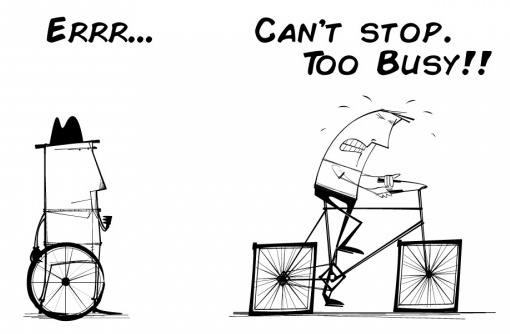
\includegraphics[scale=0.5]{img/toobusytoimprove.jpeg}


\section{State of Art }

As part of the research process has been analyses some aplications
that (although isn't a directly competition) represent the actual
state of art about the kind of sofware we are talking about.


\begin{table}[]
\centering

\begin{tabular}{@{}lllllll@{}}

Feature & classDojo & TeacherKit & A+ & iDoceo & Additio & SMS \\ \midrule

Attendance & \completeValue & \completeValue & \completeValue & \completeValue & \completeValue & \completeValue \\

Discipline & \partialValue & \completeValue & \completeValue & \completeValue & \completeValue & \completeValue \\

Attitude & \partialValue & \completeValue & \completeValue & \completeValue & \completeValue & \completeValue \\

Marks & \noneValue & \completeValue & \completeValue & \completeValue & \completeValue & \completeValue \\

Competencias & \noneValue & \noneValue & \noneValue & \completeValue & \completeValue & \completeValue \\

Rubrics & \noneValue & \noneValue & \noneValue & \completeValue & \completeValue & \completeValue \\

Message & \completeValue & \completeValue & \completeValue & \noneValue & \noneValue &	\completeValue \\

patters & \noneValue & \noneValue & \noneValue & \completeValue & \completeValue & \completeValue \\

reports & \noneValue & \completeValue & \completeValue & \partialValue & \completeValue & \completeValue \\

analysis & \partialValue & \completeValue & \partialValue & \partialValue & \partialValue & \completeValue \\

models and predictions & \noneValue & \noneValue & \noneValue & \noneValue & \noneValue & \completeValue \\

Centralizate and jerarqy & \noneValue & \partialValue & \noneValue & \noneValue & \noneValue & \completeValue \\ \midrule

Total & 58.3\% & 80.5\% & 72.2\% & 	72.2\% & 80.5\% & 99\% \\
\end{tabular}
\caption{Features}
\label{my-label}
\end{table}


\begin{table}[]
\centering

\begin{tabular}{@{}lllllll@{}}

Feature & classDojo & TeacherKit & A+ & iDoceo & Additio & SMS \\ \midrule

Personalization & \noneValue & \noneValue & \noneValue & \noneValue & \noneValue & \noneValue \\

Good UI & \partialValue & \completeValue & \completeValue & \completeValue & \completeValue & \completeValue \\

Buena UX & \partialValue & \completeValue & \completeValue & \completeValue & \completeValue & \completeValue \\

Price & \noneValue & \completeValue & \completeValue & \completeValue & \completeValue & \completeValue \\

Performance & \noneValue & \noneValue & \noneValue	 & \completeValue & \completeValue & \textcolor{ownGreen}{\completeValue} \\

Scalable & \noneValue & \noneValue & \noneValue & \completeValue & \completeValue & \completeValue \\

Data control & \completeValue & \completeValue & \completeValue & \noneValue & \partialValue & \completeValue \\

Multiplatform & \noneValue & \noneValue & \noneValue & \completeValue & \completeValue & \completeValue \\

Centralized & \noneValue & \completeValue & \completeValue & \partialValue & \completeValue & \completeValue \\ \midrule

Total & 44.4\% & 50.0\% & 16.6\% & 	16.6\% & 44.4\% & 99\% \\
\end{tabular}
\caption{Architecture and design}
\label{my-label}
\end{table}


\chapter{Designe Decisions }

Nowadays we can build almost any kind of software with a lot of differents
language from which to choose, but as if that were not enough there
are also a lot of architectures that are possible to follow, and beside
of this it will necesary choose where deploy our software, or how
doc it, or how magane our work team, etc. A lot of options that it
will necesary to choose and that can make the difference between the
success or failure of our project. So, what about of these decisions
in this project? Take a look about it.

\section{Kind of software}
Based of informal requirements was thinked that the best option must be a \textbf{web app} for a lot of reasons. First of all because is the simplest way to offer an app that can run in almost any device (with a \textit{simple\footnote{Actually a browser is one of the more complex pieces of software, but here is labeled as simple because is a software that the mayority of device like smartphones, tablet, etc, have by default and for the most non technical people isn't a complex software, nothing could be further from the truth.}} browser). 

\section{Architecture}

\subsection{Why microservices?}

Much more that the trend in the develop of apps, all of change of
paradigm inspired in distributed system, now over http and focussed
(especially) in web apps as a consequence of the multiple benefits
to this kind of sofwate. \bigskip

Language agnostic, scalable, size ajustables, independently, the system
splited in litle pieces with this boundaries ...

\subsection{Why polyglot database?}

With the mircroservices approach the system will be some very differents
database to do some diferents things. So, in general we can see our
backend like a black box when the data persists in a polyglot database.
That means that the data is save in differents ways, using diferetns
formats and diferents driver to manage this. There are a group of
data that it need saved with certain relations, due to its nature,
so a relational database seem perfect to do this, but this kind of
databases (like MySQL) can been slowly or too heavy for other tasks
of kind of processes, like data analysis.

\subsection{Repository Strategie}

\section{Languages and frameworks}

\section{Deploy scenarios}

Google App Engine, Amazon Web Services, Microsoft Azure, IBM BlueMix,
Heroku, CloudFoundry, etc...

Realizar comparativa y justificar muy bien la eleccion.

\section{Documentation}

\section{Methodology and planification.}

Eleccion de metodologias agiles basadas en Scrum para la gestion del
equipo y en historias de usuario para el modelado del sistema.

\subsubsection {ds}

\section{License}

\subsection{Licencia y enfoque}

\chapter{Architecture Modeling}

En base a los requisitos funcionales del sistema, se ha modelado la
arquitectura en base a ciertos subsistemas o microservicio

2

\section{General Patterns}


en microservicios, entre ellos el basado en una API GATEWAY que es
el adoptado por nosotros.

\section{Evolution}

En muchas ocasiones lo más interesante de un desarrollo, la fase propia

En este caso se pierden las conclusiones y decisiones tomadas por
el equipo de desarrollo que les han llevado a toma una u otra decisi
Por eso se intentará reflejar lo más fielmente posible como ha sido
el proceso que ha llevado el sistema al su fase de entrega final.

\subsection{First Phase}

Servicios básicos y no demasiado estandard

\subsection{Second Phase}

Los microservicios básicos

\subsection{Third Phase}

La arquitectura final

\subsection{Not closed final state}

Estado final pero por supuesto no cerrado al cambio ni a la ampliac
con los servicios que faltarían o que no estan aún externalizados.

\chapter{Core}

Talking about SPIKES in all sections that is needed, como UIKIT en
la UI, endpoints en la APIG, ndb, mongo, etc, etc...

\section{APIGmS}

\subsection{Introduction}

As has been comment before, the pattern choose to this microservices
based app architecture is API Gateway, this offers a lot of benefits,
but also some drawbacks. The mainly idea is to have a service working
like as the gateway of the service, so the backend becomes in a black
box where all inside is behind of this service, transparent to the
customers of this.

So, this service works basically like a dispatcher, it receives the
calls from user interface and decide where send the request.

\subsection{Spikes}

To build this services was tryed some diferents approach. Like almost
in every modules, the same functionality can be writed for may ways.
So, in this case specially (a service thinkied to run in GAE) the
platform offer us a speciall way to do this, better than standard,
according to them.

\subsection{Testing and docs}

As is a dispatcher, the testing strategie isn't like others. Don't
have sense write (be automatic or not) a lot of test that redo the
same checks only using another port (in local) or url (in production).
To do this easier, a simple strategie is execute the same test that
are executed over the microservices isolated from the APIGmS, exactly
the same.\bigskip How do this? The tests writed uses a url that included
a port of execution (because all servies using the same url in local)
so if we want to know if the response is equal from APIGmS we only
need change the port of execution. So, for example if the tests suite
to serviceA runing over localhost:8003 the test that check this service
throught APIGmS (must be exactly the same behaviour) will use localhost:8001.

The tool used to do all test (except for the UI) is the python framework
PyTest allow easily, writing scenarios. This technique allow repeat
all test first over the service and after from the distpacher (showing
all result as well).

Besides of this, the service can have functions of modules that need
be tested independently, these need a specific tests.

\bigskip

On the other had with docs something similar happens, don't have sense
write a doc defining the behaviour of all sections of api gateway
if this doc already exists in each service. It's redundant and complex
to mantain. Because of this a simple approach is link the docs to
services docs, so the task of write it relegate to them.

As is saided the tool Sphinx is used to build the doc of the service.
That basically inspect the code files mixing this with all the files
that we write (pure doc) to show this as a web based documetnation
(easy to read and understand).

\section{TDBmS}

\subsection{Introduction}

This mService offers the managment of the teaching of the center.
This means that persist in a relational database all relations between
teachers, students, subjects, etc, and all resource availables to
make this posible throuhg an api.\bigskip

This like the rest offers his resource throuhg an api writed in Flask
(follow the same architecture that all).

The engine to save all these relations is MySQL, for many reasons,
mainly because is the best known engine and in which it has some experience
and also because GCP offers as a cloud product Google Cloud SQL Databases.
Until recently only offerts MySQL but now (since March of 2017) they
offer also PostgreSQL.

\subsection{User stories}

As base of requirements process have been used user stories.

\noindent\shadowbox{\begin{minipage}[t]{1\columnwidth - 2\fboxsep - 2\fboxrule - \shadowsize}%
\textbf{\#1 }

Me as manager, I want save subjects, teachers, students and classes.%
\end{minipage}}

\bigskip

\noindent\shadowbox{\begin{minipage}[t]{1\columnwidth - 2\fboxsep - 2\fboxrule - \shadowsize}%
\textbf{\#2}

Me as manager, I want can relate teachers with subjects.%
\end{minipage}}

\subsection{Design}

\subsubsection{E/R designe}

Based on user histories and the domain of the problem the designe
done based of this entity relation diagram:

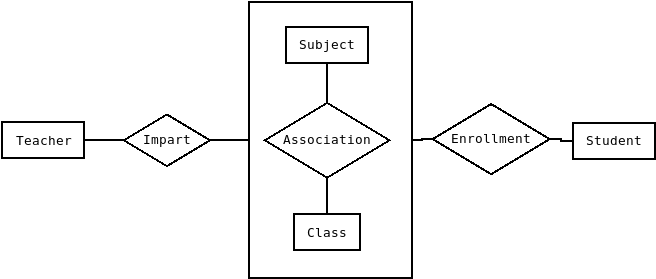
\includegraphics[scale=0.5]{img/diagrams/dbms-ER}

The design follow some details that the domain presents, that is related
(at least the more significantly) below:

\subsubsection{Access Library}

In the old version it was a little ORM that offers simple methods
to access data transform this in SQL raw sencentes. Now this library
is only a wraper of the SQLAlchemy to keep apart the apirest of the
service to the database access layer.

\subsubsection{mService API}

\subsection{Stones and evolution}

\subsubsection{Way to access to raw data}

While at firs of develop the mainly strategie to follow was write
all by cero, finally the point of view has been changed to follow
the use of standard tools and avoid reinvent the wheel.

So, if in the first stages of the project the acces to raw data through
the engine was hand made, using an own simple library that worked
like as simple ORM, the evolution of it and especially the problems
found and the unmaintainability of code have made that now the approach
turned to use a good tool as ORM like \href{http://www.google.es}{SQLAlchemy}.

The changes in the specifications of the api while the develop and
the maintaince of the performance of the queries when is writed hand
made in raw SQL isn't a good idea. Before the develop of this mService
it easy to understand that only in few projects is justified the use
of raw sql sencences and drivers whiout ORM (by easy that it was).

\subsubsection{Delete items strategy}

dfasdf

\subsubsection{Item's metadata.}

\subsubsection{Input / Output convention}

All in JSON except the values with NULL in the input and in the output.

\subsubsection{How to save the deleted items.}

In the way to develop the microservice we have the question, we want
to save the deleted items? For one hand we could want to know

\subsubsection{Optional subjects, the ``class'' Table.}

In the domain of the problem can be exists optative subjects and is
needed search a way to implement this because has a specific details
that aren't like the rest.

\paragraph{The details.}

The studies plan forces in certain courses to select one or several
optional subjects. For example, if a student has enrollment in 2ºESO
(independently of the group, A, B...) the law and consequently the
studies plan force to the student to choose between some optional
subjects. So, maybe this subjects exists only in this optional case
as `` rare subjects'' but in other cases this are only normal subjects
but that in this course are offer like optional.

A simple example of this is French subject, it in some courses like
3ESO and 4ESO is obligatory but it in Bachiller (the upper level)
is optional because the students can be select if they want make the
final exam with this second language or select another like English
or Greek or Latin p.e.

To obtain this we decide develop a simple solution without change
the original database logic schema. So, how we have an entity that
save the classes and it have three attributes, course, word and level
mainly we going to add three more to this special cases, optative,
groupNumber and subgroupNumber. Like this special cases haven't word
param when they have value word don't have and when the item have
word (A, B, C...) then don't have this special attributes.

Maybe this don't be the best solution, but is a simple in the point
of develop.

Obviously like we can't have two autoincrement values in the same
table definition in MySQL we will need control this programatically,
but is something that we can assume to get our goal easily.

Problema:

La misma ventaja que nos ofrece UNIQUE para el caso de los eliminados
ahora nos muerde aquí. Mientras que allí beneficiaba porque esta clausula
no incluye a los item que tengan campos a null y permite que no de
conflicto en este caso si insertamos un grupo optativo obviamente
deberá tener el camo word a null y si es así podemos tener exactamente
dos grupos iguales sinque de conflicto.

course

1 <null> ESO 1 1 1 0

1 <null> ESO 1 1 1 0

Sin dar conflicto, lo que no puede ser.



está a null o no para le resto de los procedimientos.

Por esta razon decidimos usar el mismo campo word, con una nomenclatura
especial, ya que no se va a ser usada para los grupos generales que
indique que se trata de un grupo optativo y además especifique el
grupo y el subgrupo, en concreto:

OPT\_n\_m

donde n será el número del grupo (que habrá que incrementar prograticamente
a mano) y m el número del subgrupo que tambi\'{n}e habrá que incrementar
a mano en caso de que se creen más.

Esto siempre a falta de un mejor solucion que se adopte en iteraciones
posteriores.

Y en la api nosotros siempre preferimos explícito a implicito.

Requisitos:
\begin{enumerate}
\item Ya que todo se controla desde mysql pero no existe forma de hacerlo
automatico vamos a crear unos disparadores para la inserccion y la
eliminacion para mantener la consistencia de los datos. Cuando se
introduce un nuevo grupo optativo se debe comprobar que existe el
anterior tanto en grupo como en subgrupo para que no exista el subgrupo
4 sin el 3 o el dos. De la misma manera no se podrán eliminar un grupo
4 si el 2 aún existe.
\end{enumerate}

\paragraph{API definition}

@app.route('/entities/<string:kind>', methods={[}'POST'{]})

Para realizar la introduccion de un estudiante al sistema usamos

el re.

No podemos introducir un usuario que no tenga datos, al menos

deberá pasarse el dato nombre que es úniquo mínimo que debe

existir para el tipo alumno.

Cuando se pide una lista de elementos y la peticin se realiza correctamente
pero no se devuelve nada porque no existen items de ese recurso se
envía un 204 Success without content.

Importante: Muchos de los detalles de control de consistencia no pueden
relegarse a la UI, ya que aunque en ella no se deben permitir ciertas
acciones por la logica del sistema, la api no debe permitir su realizacin
aunque se haga de forma manual sin los conectores de la UI.

Por eso no solo la seguridad sino el control de la consistencia debe

estar presente de la mejor forma posible en todas las acciones que
contra esta un usuario puede hacer.

\paragraph{User histories}

El microservicio de Base de Datos acota el dominio de la gestin docente
dentro del sistema, quizs se le cambie el nombre a TmS teachingMicroService.

A través de este microservicio podemos realizar todas las acciones
relativas a.

Este microservicio se basa en una base de datos.

I like

\section{SCmS}

\subsection{Introduction}

Students Control micro Service or SCmS is the service that provide
the resources to make posible tasks like .... .

All of this working independently to the rest of the system with her
own database.

\subsection{User Stories}

sdfsdfds

\subsection{Deficiencies Analysis}

\subsubsection{D1}

Deficiencias el proceso posterior a la corrección de un examen.

Un profesor cualquiera (A en este caso) corrige un curso de exámenes (30 por ejemplo) y después pasa las notas a una libreta/cuaderno que les suministra el centro. Esto solo como lugar intermedio de registro, y aque después es necesario pasarlo al sistema SENECA (externo).
El profesor para de media 10 min haciendo solo el paso de las notas a su libreta y otros 5 min en hacer el paso a SENECA. Un total de unos 12/14 min de media de trabajo extra que no aporta ningún valor al proceso de correción de exámenes.

Además de esto, existen muchos datos que se pierden por la forma de procesar los datos. 

Imaginemos que el profeso quiere saber la nota media que el curso ha sacado en ese examen, debería de calcularla a mano, o compararla co nuna notar de un examen anterior (ya sea a nivel de grupo o a nivel individual). O por ejemplo quien ha sacado mejores notas, si los chicos o las chicas, o cierto grupo de control con otro. 

Por otra parte se hace imposible el acceso a procesamientos más complejos como lo que podría ofrecer el sistema:

Puedes comparar la nota de un persona porque al anotarla tienes su nota anterior al lado, pero y si quieres ver la evolución general del grupo no puedes.
¿Y si quieres ver que competencia de ese examen ha salido mejor o peor? Como que se les ha dado mejor, si la parte de redacción o la parte de listening, por ejemplo, para esto se podrían registrar más notas a parte de el simple resultado general del examen. Pudiendo hacer un sistema muchísimo más 
potente para el análisis de datos de estudiantes y así su mejora.

Eleva la potencia del examen por mil.






\subsection{First Iteration}

Like in every scenarios we can divide the domain of the problem in
some services, but in this

case and like first iteration it has been decided leave toguether
all the issues thar are related with the students controls.

\subsection{Designe}

\subsubsection{Arquitecture}

\subsubsection{Languages and tools}

\subsection{Testing strategy}

\subsection{Deploy}

\section{AmS}

\subsection{About}

Analytics micro Service or AmS.

\subsection{First Iteration}

\subsection{Designe and arquitecture}



\subsubsection{Languages and tools}

\subsection{Testing strategy}

\subsection{Deploy}

\section{UImS}

\subsection{Scope}

\subsection{UX basic strategy issue}

Explicacin del problema.

\subsubsection{All in one}

Cuando todo se trata como un boque al que se le procesan las diferencias.

\subsubsection{All live mode}

Donde por cada accin se realiza una llamada a la api y no existen
los botones guardar, incluso cuando se escribe texto en los campos
se está realizando el guardado.

\subsubsection{Mixed mode}

Donde la seccion de datos propios de la entidad se procesa de forma
tradicional y las relaciones se actualizan conforme se manipulan.
Esta es la que finalmente optamos por usar.

\section{External Services}

Conclusiones de por qué se han usado ciertas cosas y por que no otras

\subsection{Pub / Sub pattern}

\subsection{Firebase}

\subsection{Third Party DataBases}

Por que nos hemos quedado con las que usamos y porque no usamos otras.

\chapter{Future Plans}

\section{Features}

\section{Architecture}

Image of all microservices in their final state

\section{Technologies}

\chapter{Retrospective}

Solo ahora que va acabando el proyecto es posible ver todos los problemas
que se han tenido y la forma de ponerles solucin de una forma +
amplia, viendo donde se cometieron erroes y cuales han sido los beneficios
y cuellos de botella del desarrollo del proyecto.

\section{DRY}

Comentar algunas de las cosas en las que se ha caido, como el escribir
cosas desde cero cuando habías soluciones o cosas parecidas ya hechas.

La validacin de envíos en las apis, los ORMs, la documentacin, el
testing, etc, etc...

\section{KISS}

\section{The heaven of frameworks}

Existen un monn de frameworks distintos para hacer lo mismo, cada
uno en su lenguaje, y cada uno con sus detalles. ahora que terminamos
el proyecto, evaluamos los beneficios y problemas que hemos encontrado
en unos y otros, atendiendo entre otras cosas a la demanda y uso d
elos mismos, desde el número de oportunidades laborales, el número
de preguntas en stackoverflow .

\section{Community}

el contacto con la comunidad, debería de haber sido mucho mayor y
previo, (comunidades profesionales)

\section{The strategie}

Los problemas de la planificacin, las virtudes de hacer algo as,
lo aprendido con las historias de usuario y como es muy dificil abordar
un problema de este tamao solo, la dificultad de encontrar colaboradores,
etc, etc...

\section{DevOps and storms in the cloud}

Conocimientos, lugares donde desplegar, infrastructura de google,
los problemas que se han encontrado, como diferencia esto de un despliegue
en otro sitio (en cuanto a curvas de aprendizaje).

\chapter{Achievements}

This project, whitout to be the most innovation project has been enough interesentign (for any reason) to give some profesional oportunities. 

For one hand, this project has been enrolled in the Talefonica Talentum Program (2016 Edition), give us the oportunity to join to an interdsiciplinar group of people (students of Computer and Telecomunications Engenier), some one with own project, shanring experiences and work. Finally this porject wasn't selected to the next phase, another projects with more commercial projection that a open source project was more interesting, for oviously reasons. But he experience was really interesting and (motivadora). 

For other hand and most important, the oportunity to join to a really interesting StartUp in Granada. This young company named CocktaiLabs saw this project in the list of project enrollment in Open Project OSL Contests 2016-2017 and (se puso en contacto) with the main autor, offer it hire it, to join in a develop group to build a system that share some ideas with the project developed to the contest and explained here.

Beside of this, the born of this project and the iinmersion in the open source concept also did that if formed a open source developers group (Butterfly Devs) where some friends join kwowlements working in some projects 


\chapter{Resources }

\section{Articles}
\begin{enumerate}
\item http://blog.zachbjornson.com/2015/12/29/cloud-storage-performance.html
\item http://googlecloudplatform.blogspot.com.es/2015/12/the-next-generation-of-managed-MySQL-offerings-on-Cloud-SQL.html
\end{enumerate}

\section{Communities}
\begin{enumerate}
\item https://plus.google.com/+googlecloudplatform/posts
\item https://plus.google.com/+AngularjsEspa\%C3\%B1ol/posts
\end{enumerate}

\section{Technologies}
\begin{enumerate}
\item https://material.angularjs.org/
\end{enumerate}

\section{Books}

\chapter{Acknowledgments}

Special acknowledments to my family, for all time (invertido) on mine, the (patient) and for their ehternal and infine support. Of course also to Susana, for her pattient with me, (a pesar) of not understand (all that I do). Speciall mention to JJ. Merelo for the oportunity to work with him (elevating this projecto to other level of concpet and profionalidad) and JJRamos (mentor of Telefonica Talentum Program) for all their energy, (animo), entusiasmo contagioso y por todos los buenos ratos que hemos pasado trabajando (entre otras cosas). 

And another list of people that (de una forma u otra and ayudado conceptualmente al projecto).


Alan O'Rourke por la imagen de toobusy toimprove

\begin{itemize}
\item Al resto del equipo de ButterFlyDevs, Jose Antonio Gonzalez y Alvaro Maximino Herrera por sus esporádicas pero inestimables contribuciones al projecto.
\item Ignacio Zafra (The Cloud Gate)
\item Alberto Guillen
\item Esteban Gomez Roldan (GDG Granada)
\item Steve Judd (OpenCredo LTD)
\item Victor Terrn (Google London)
\item Nacho Coloma (Extrema Sistemas)
\item José M. Rodríguez (Job\&Talent)
\end{itemize}
\bibliographystyle{plain}
\nocite{*}
\bibliography{books}

\end{document}
